\section{Theory}
In this repport we are working with the Fresnel relations, which describe the amount of $s$- and $p$-polarized light transmitted and reflected at the boundary of a dielectric surface. Generally we remind ourself of the relation between the angles of the incoming light $\theta$, the reflected light $\theta_1$ and refracted light $\theta_2$. The angles are measured from the normal of the dielectric surface.
\fxnote{insert reference}
The relation between the incoming and reflected beam is given by the simple relation:
%
\begin{align}
\theta = \theta_1
\end{align}
%
The relation between the angles of incidence and refraction is given by Snells' law:
%
\begin{align}
n_1\sin{\theta}=n_2\sin{\theta_2}
\end{align}
%
where $n_1$ and $n_2$ are the refractive indices of the materials at the boundary of the incoming and reflected light beam.

\subsection{Polarization}

The plane spanned by the normal vector to our dielectric surface $\hat{\textbf{n}}$ and the wave vector $\textbf{k}$, which is in the direction of the propagation of the light, is called \textit{the plane of incidence}. The direction of the $\textbf{E}$-field relative to this plane then determines the polarization of the light, if $\textbf{E}$ is parallel to the plane of incidence the light is $p$ polarized and if $\textbf{E}$ is perpendicular to the plane of incidence then the light is $s$-polarized. 
%
\begin{figure}[h]
    \centering
    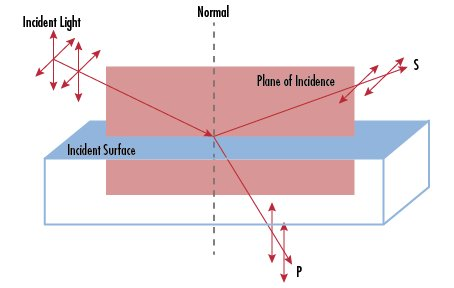
\includegraphics[width=\columnwidth]{plane}
    \caption{P and S linear polarizations defined by their relative orientation to the plane of incidence.}
    \label{fig:planeofincidence}
\end{figure}
\noindent
Light from normal light sources has a mixture of all possible directions of polarization but the generally any polarization can be given as a linear combination in a basis of electric field with $s$- and $p$-polarization. Using a polarizer one can filter one kind of polarization of a beam.

\subsection{Fresnel relations}
%THIS IS JUST A DRAFT!we'll have to check Griffiths to see if i make any sense
When a beam of light interacts with the surface of a dielectricum a certain percentage of the light will be reflected as well as transmitted. The percentage of light reflected is denoted $R$ and the percantage transmitted is denoted $T$. As the light is either transmitted or reflected it is natural to conclude that:
%
\begin{align}
R+T=1
\end{align}
%
To make things easier for ourselfes we define $R=r^2$ and $T=\frac{n_2\cos{\theta_2}}{n_1\cos{\theta_1}}t^2$ where $r=\frac{E_1'}{E_1}$ and  $t=\frac{E_2}{E-1}$ with $E_1$ denoting the magnitude of the incoming $\textbf{E}$-field, $E_1'$ denoting the magnitude of the reflected $\textbf{E}$-field and $E_2$ denoting the magnitude of the transmitted $\textbf{E}$-field. As the direction of the $\textbf{E}$-field can be written in the basis of $s$- and $p$-polarization we can define our reflection and transmission indexes for $p$ and $s$ polarized light seperately. Our $r_p,r_s,t_p$ and $t_s$ given as functions of $\theta_1$ and $\theta_2$ are:

%Find more details
\begin{align}
r_p = & \frac{n_{2}\cos(\theta_1)-n_1\cos(\theta_2)}{n_2\cos(\theta_1)+n_1\cos(\theta_2)} = \frac{\tan(\theta_1-\theta_2)}{\tan(\theta_1+\theta_2)}\\
%
t_p = & \frac{2n_1\cos(\theta_1)}{n_2\cos(\theta_1)+n_2\cos(\theta_2)} 
= \frac{2\cos(\theta_1)\sin(\theta_2)}{\sin(\theta_1+\theta_2)\cos(\theta_1+\theta_2)}\\
%
r_s = & \frac{n_1\cos(\theta_1)-n_2\cos(\theta_2)}{n_1\cos(\theta_1)+n_2\cos(\theta_2)}= -\frac{\sin(\theta_1-\theta_2)}{\sin(\theta_1+\theta_2)}\\
%
t_s = & \frac{2n_1\cos(\theta_1)}{n_1\cos(\theta_1)+n_2\cos(\theta_2)} = \frac{2\cos(\theta_1)\sin(\theta_2)}{\sin(\theta_1+\theta_2)}
\end{align}
%
Then we find:
\begin{align}
R_p = & \frac{\tan(\theta_1-\theta_2)^2}{\tan(\theta_1+\theta_2)^2}\\
T_p = & \frac{\sin(2\theta_1)\sin(2\theta_2)}{\sin^2(\theta_1+\theta_2)\cos^2(\theta_1-\theta_2)}\\
R_s = & \frac{sin^2(\theta_1-\theta_2)}{\sin^2(\theta_1+\theta_2)}\\
T_s = & \frac{\sin(2\theta_1)\sin(2\theta_2)}{\sin^2(\theta_1+\theta_2)}
\end{align}

	







